\chapter{Introduction}
\label{chapter:intro}

Innovation--what is it and why it is important? Innovation refers to the ability to create and capture economic value from invention \citep{Hagel2005TheSpecialization}. Innovation is key driver of any sustainable business and, indeed, society. Innovation has become an imperative for business, academic and governmental organizations in response to environmental and technology-driven changes \citep{Drucker2015InnovationPrinciples,VandeVen1986CentralInnovation,Gupta2007InnovationAnalysis,Schumpeter1942CapitalismDemocracy}. \cite{Carlson2006}, among others, underline the imperative role of innovation: ``Nothing is more important to business success than innovation.'' Over the past century, conceptual approaches for understanding and accelerating innovation have evolved. 

What are innovation ecosystems and why are they relevant in 2016? More often than ever before, innovation is taking place outside and in between individual organizations. Moreover, consumers now have an active role in innovation, i.e. in value co-creation. Through open innovation and value co-creation, several steps have been taken from manufacturing-driven, technology-push view \citep{Schumpeter1934TheCycle,Schumpeter1942CapitalismDemocracy,Schumpeter1950TheSocialism} to that of the ecosystemic view both to business and innovation \citep{Russell2011TransformingOrchestration,Moore1993PredatorsCompetition,Jarvi2013}. \cite{Autio2013InnovationManagement} define innovation ecosystem as ``a network of interconnected organizations, organized around a focal firm or a platform, and incorporating both production and use side participants, and focusing on the development of new value through innovation.'' \cite{Russell2011TransformingOrchestration} take an even broader view to define innovation ecosystem as an ``inter-organizational, political, economic, environmental and technological systems of innovation through which a milieu conducive to business growth is catalyzed, sustained and supported.'' In system level, individual relationships take the shape of a network ``through which information and talent flow through systems of sustained value co-creation.'' \citep{Russell2015RelationalEcosystems}

Key influence in the adoption of the ecosystem concept in the context of innovation is the concept of business ecosystem that \cite{Moore1993PredatorsCompetition} introduced. Ecosystem is used in this context both as a metaphor \citep[e.g.][]{Hwang2012}, a strategy artifact \citep{Moore1993PredatorsCompetition}, as well as to refer to system-level analysis \citep[cf.][]{Pentland2015}. 

Innovation ecosystems are rather orchestrated than controlled or managed \citep{Russell2011TransformingOrchestration,Ritala2009,Ritala2013}. When collective gains are sought at the network level, change agents seek to facilitate the emergence of networks, orchestrate existing networks and manage their growth \citep{Russell2011TransformingOrchestration}. To manage innovation ecosystems as well as to facilitate their emergence, the process of network orchestration is encouraged \citep{Russell2015RelationalEcosystems}.

Why visual network analysis is valuable in exploring innovation ecosystems?

\begin{quote}
``Use a picture. It's worth a thousand words.'' -Arthur Brisbaine \citep{Bendoly2016FitAnalytics}
\end{quote}

\begin{quote}
``...few people will appreciate the music if I just show them the notes. Most of us need to listen to the music to understand how beautiful it is. But often that’s how we present statistics; we just show the notes we don’t play the music.'' - Hans Rosling 
\end{quote}

In this dissertation, innovation ecosystems are investigated with visual network analytics approach. From the beginning of social network analysis and its precursor sociometry, visualization has been a key part of the analysis process, cf. \cite{Moreno1953}:
\begin{quote}
``We have first to visualize [...] A process of charting has been devised by the sociometrists, the sociogram, which is more than merely a method of presentation. It is first of all a method of exploration. It makes possible the exploration of sociometric facts. The proper placement of every individual and of all interrelations of individuals can be shown on a sociogram. It is at present the only available scheme which makes structural analysis of a community possible.''\end{quote}

Explorative visual analysis of networks and therefore ecosystems allows holistic investigations as well as sharing the findings to others \citep{Freeman2000VisualizingNetworks}. The challenges and opportunities of visualization in general and  visual network analytics specifically have received little attention in innovation ecosystem research. \cite{Basole2014} states that while research on challenges and opportunities of visualization in corporate settings exists \citep{Lam2012,Sedlmair2011}, ``researchers haven’t focused on visual business ecosystem intelligence tools.'' The observation also applies to innovation ecosystems.\footnote{Innovation Ecosystems Network is among the first to contribute to the field of visual innovation ecosystem analytics through \href{http://www.innovation-ecosystems.org/2011/05/31/ies2011/}{Innovation Ecosystems Summit (2011)}, \href{http://www.tut.fi/iislab/fi/2011/09/23/visualizing-innovation-ecosystems-mindtrek-2011/}{Visualizing Innovation Ecosystems workshop} at Mindtrek 2011 and \href{https://ien.stanford.edu/hicss2016}{Analytics and Decision Support for Ecosystems} Minitrack at HICSS 2016.} In all, empirical research on innovation ecosystems is scarce and this is particularly true to in ecosystem-level (rather than in actor or relationship level) \citep{Jarvi2016TakingReview}.

Why should these explorations and investigations be conducted with a data-driven, computational approach? New ways to measure innovation are needed \citep{Still2012ParadigmDigital}. Social media, socially constructed datasets and other sources of digital data create a plethora of new opportunities for measuring activities particularly toward the upstream of innovation. At the same time, using social media as a source for measuring innovation is far from straightforward \citep{Salonen2013ChallengesMedia}. The objective of this dissertation is to develop essentially a new research method for data-driven investigations of the structure of innovation ecosystems. The method falls under computational social science \citep{Lazer2009ComputationalScience}.

With more recent theories and paradigms such as the network-driven nature of the world \citep{Watts1999,Barabasi2003} and, more recently, computational social science \citep{Lazer2009ComputationalScience} and social physics \citep{Pentland2015}, the anticipation of the possibility to develop theories for human behavior that are nearly as specific as in physics or natural science is growing in a number of domains. The machinery, however, is at its infancy during the time of writing this dissertation. In the investigations we conduct for the dissertation, we focus in finding the kinds of datasets that would give us a similar system-level view into innovation ecosystems \citep[cf.][]{Pan2012}.

From these grounds, we began our venture in 2010 to investigate how social media and other publicly available data sources to map, analyze and visualize the network structure of innovation ecosystems. In this dissertation, we take a data-driven approach to visual network analytics. Here, data-driven means that the analysis process relies on data, is automated and conducted in a computational manner. Additional data can augment the dataset selected for analysis through an automated software process. Established analytical procedures can be automated, yet new conditions for analysis-based insights can be introduced and refined incrementally with continuous computational iterations. We will revisit the development of these procedures in Chapter~\ref{ch:processmodels}.

Drawing from our experience in running multiple experiments in the context of exploratory and descriptive innovation ecosystem investigations, we take a Action Design Research (ADR) \citep{Sein2011ActionResearch} approach to describe a process model for data-driven visual network analytics.

\section{Objectives of the dissertation}
\label{sec:objectives}

This dissertation targets the research gap in ecosystem-level innovation ecosystem investigations. First, as \cite{Jarvi2016TakingReview} point out, empirical studies on innovation ecosystems are scarce in general and in particular in ecosystem level. Moreover, visual analytics tools and methods for studying innovation ecosystem structure are largely missing \citep[cf.][]{Basole2009VisualizationEcosystem}. We answer Freeman's \citeyear{Freeman2000VisualizingNetworks} call to develop an integrated method to retrieve social network data, create networks, compute network metrics and to visualize networks. Finally and most importantly, we take into account the requirements and limitations stemming from the development and use of visual network analytics tools for innovation ecosystem investigations taking place in their natural habitat, i.e. in interdisciplinary teams that, according to \cite{Bendoly2016FitAnalytics} seek ``not just simultaneous parallel use [of data and visualizations] but truly joint utilization and team-wise sensemaking for effective decisions.''

The overall objective of this dissertation is to develop means to investigate innovation ecosystems as networks through visual analytics. We claim that representing innovation ecosystems as networks is particularly intuitive and expressive in supporting their exploration and in allowing for a system-level view.

More specifically, the individual objectives of this dissertation are summarized as follows:

\begin{enumerate}[label=\textbf{Objective \Roman*},align=left]
	\item To contrinute to the empirical body of knowledge on innovation ecosystems through modeling and visualizing the network structure of a set of innovation ecosystems of different levels of abstraction and complexity.
    \label{objective:empirical}
	\item To identify patterns for modeling and analyzing the structure of innovation ecosystems as networks.
    \label{objective:ecosystemnetworks}
	\item Finally and most importantly, to define a process model for data-driven visual network analytics of innovation ecosystems.
     \label{objective:processmodel}
\end{enumerate}

In the next two sections, we will comment on the philosophical foundations of the dissertation and discuss in detail the research methodology applied in this dissertation to reach the objectives.

\section{Research methods and restrictions}
\label{sec:methods}

This dissertation falls under the domain of Information Systems (IS) research. IS researchers seek to develop means to create value out of information for people, teams, and organizations \citep{Nunamaker2011TowardSystems}. Due to the wide scope of knowledge IS is drawing from, \cite{Nunamaker2011TowardSystems} urge IS researcher to ``embrace multi-investigator, multidisciplinary, even multiuniversity research teams.''

The field of Information Systems is an example of the science of artificial \citep{Simon1969} in which the objectives of investigations are man-made artifacts rather than phenomena in nature. Two main approaches to IS research exist. The first and more traditional is the behavioral approach where the usability, effectiveness and overall quality of already existing IT artifacts is being evaluated and measured through rigorous experiments. The second approach is to use the development process of an IT artifact to conduct research and create new knowledge. 

To solve practical problems and to create new scientific knowledge in the domain of artificial, \citep{Hevner2004} introduced Design Science Research (DSR) as a research method that allows the creation of new knowledge through the creation of new artifacts. Over the last ten years, \cite{Vaishnavi2007,Peffers2007} and others have subscribed to Design Science as a method of utility in scientific discovery. We claim that Design Science Research has a perfect fit to meet the objectives of this dissertation, i.e. to develop a) design guidelines for representing analyzing innovation ecosystems as networks (\ref{objective:ecosystemnetworks} and b) process model for supporting data-driven investigations of innovation ecosystems (\ref{objective:processmodel}.

While a large part of DSR is conducted without explicit ``discussion about underlying philosophical assumptions in the IS design science research literature'' \cite{Carlsson2010DesignApproach} and, moreover, a large part of engineering science research in general is conducted without explicit reference to its philosophical underpinnings \citep{Naukkarinen2015WhatFinland}, we will next briefly state the ontological and epistemological stance taken in this dissertation. In short, we subscribe  Carlson's \citeyear{Carlsson2010DesignApproach} proposition that critical realism provides a workable philosophical basis for Design Science Research. \cite{Bygstad2011InAnalysis} note that critical realism is an ``alternative to positivist and interpretive IS research'' and provide a straightforward definition by stating that ``Critical realism combines a realist ontology  with an interpretive epistemology'' and clarify: ``although a real world exists, our knowledge of it is socially constructed and fallible.''

Critical Realist wordview provides a firm foundation for innovation ecosystem investigations. Innovation ecosystems are open, complex, and adaptive systems \citep{Thomas2012ModelingLiteratures}. These properties yield analytic requirements that are very difficult to answer to. Critical realist philosophy allows us to establish the epistemological and ontological platform for the investigations in a way that the complexity of the phenomenon under investigation can be considered. 

We agree with \cite{Dobson2001TheResearch} in acknowledging the importance of taking a philosophical stance in establishing a common platform for investigative work. The combination of realist ontology with interpretive epistemology \citep{Bygstad2011InAnalysis} means that the investigators assume that generalizable structures and mechanisms exist in a social phenomenon. In order to identify these mechanisms and structures, however, investigators need to move beyond superficial statistical measurements and case-specific qualitative observations to apply several complementing methods, both qualitative and quantitative, in the investigations. 

More pragmatically, we point to \cite{Bygstad2011InAnalysis} who introduce critical realism as an approach to data analytics and claim that analytics process should serve the objective of identifying the structures and mechanisms that exist within phenomenon and surface as observable events. They refer to \cite{Sayer2010MethodApproach} for a layered ontology of critical realism and related research strategy that is composed of three layers: 1) events that are caused by 2) mechanisms driven by the underlying 3) structure of a phenomenon under investigation. We further agree with \cite{Dobson2001TheResearch} and \cite{Archer1995RealistApproach} in that social structure should be considered as dynamic, and therefore studying its evolution over time is important, that social structure is both a key driver of social activity, and that social activity is a key driver of the evolution of social structure. 

In the individual investigations included in this dissertation, we have applied different research approaches and methods from case study \citep{Yin2003CaseMethods} to action research and straightforward computational network analysis \citep{Lazer2009ComputationalScience}. In order to meet the objectives of the dissertation, however, the investigations serve first and foremost as experiments providing means to develop the approach for modeling the network structure of innovation ecosystems in a data-driven manner. The experiments, their context and the visual network analytics-related results are described in detail in Chapter~\ref{ch:experiments}.

Using design science research allows us to conduct research that is both 1) credible in terms of scientific theory as well as 2) has practical relevance to different innovation ecosystem stakeholders. DSR is a research method that allows “learning and investigation through artifact construction” \citep[][p.~187]{Vaishnavi2007}. In contrast to natural and social sciences where the objective is to understand reality, ``design science attempts to create things that serve human purposes'' \citep{Simon1969}. The rationale for DSR stems from the importance of the practical utility of research (\citep{Peffers2007}). Design Science aims to build a bridge between IS research and its practical application by producing results that have real-life relevance. Design Science ``creates and evaluates IT artifacts intended to solve identified organizational problems'' \citep{Hevner2004}.

Further, in terms of the different dimensions of philosophy of science, research in this dissertation is qualitative rather than quantitative (at the same time, the investigations using the produced IT artifacts are quantitative), inductive rather than deductive, and subjective rather than objective \citep[cf.][]{Olsson2012UserServices}. 
% \todo{Instrumentalism vs. relativism, see \href{http://bit.ly/1jeaObd}{http://bit.ly/1jeaObd}.} 

\cite{Sein2011ActionResearch} argue that traditional design science research prioritizes technological rigor over organizational relevance and therefore ``fail to recognize that the artifact emerges from interaction with the organizational context even when its initial design is guided by the researchers’ intent.'' To negotiate the issue, \cite{Sein2011ActionResearch} propose Action Design Research in which the research process is conducted in four stages: 1) Problem Formulation, 2) Building, Intervention, and Evaluation, 3) Reflection and Learning, and 4) Formalization of Learning. Figure~\ref{fig:adr-stages-and-principles} presents the four stages of ADR.

Three types of design are related to any IS initiative \citep{Carlsson2010DesignApproach,Aken2004ManagementRules}:
%uses van Aken's \citeyear{Aken2004ManagementRules} defines three types of designs related to any IS initiative: 
1) object design, 2) realization design and 3) process design, ``the professional’s own plan for the problem-solving cycle and includes the methods and techniques to be used in object and realization design'' \citep{Carlsson2010DesignApproach}. \cite{Carlsson2010DesignApproach} continues that: ``IS design science research should produce knowledge that can be used by the professionals in the three types of designs, including novel IT artifacts, methodologies, methods and techniques, and socio-technical implementation knowledge.''

% \begin{figure}[htb]
% \centering
% 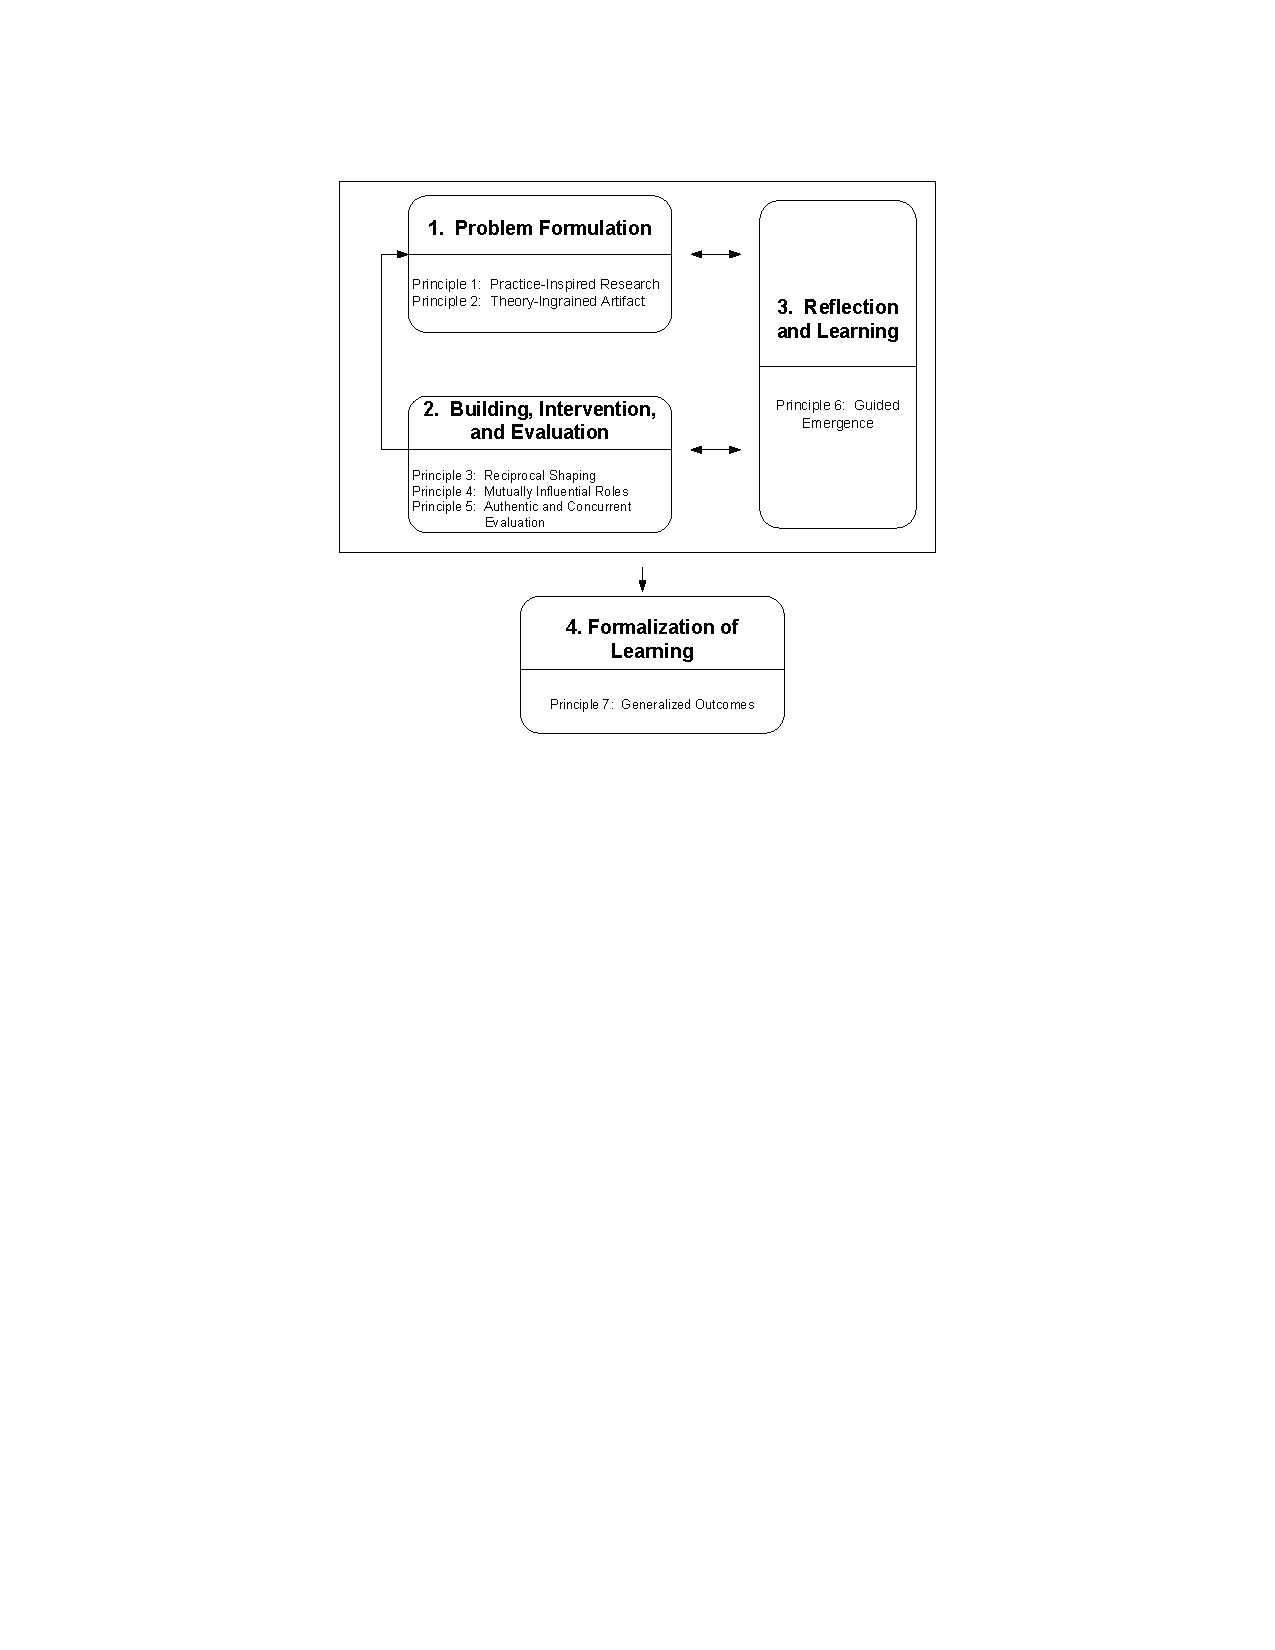
\includegraphics[width=12cm]{diagram/ADR-stages-and-principles-sein-et-al-2011.pdf}
% \caption{Action Design Research stages and principles \citep{Sein2011ActionResearch}}
% \label{fig:adr-stages-and-principles-original}
% \end{figure}

\begin{figure}[htb]
\centering
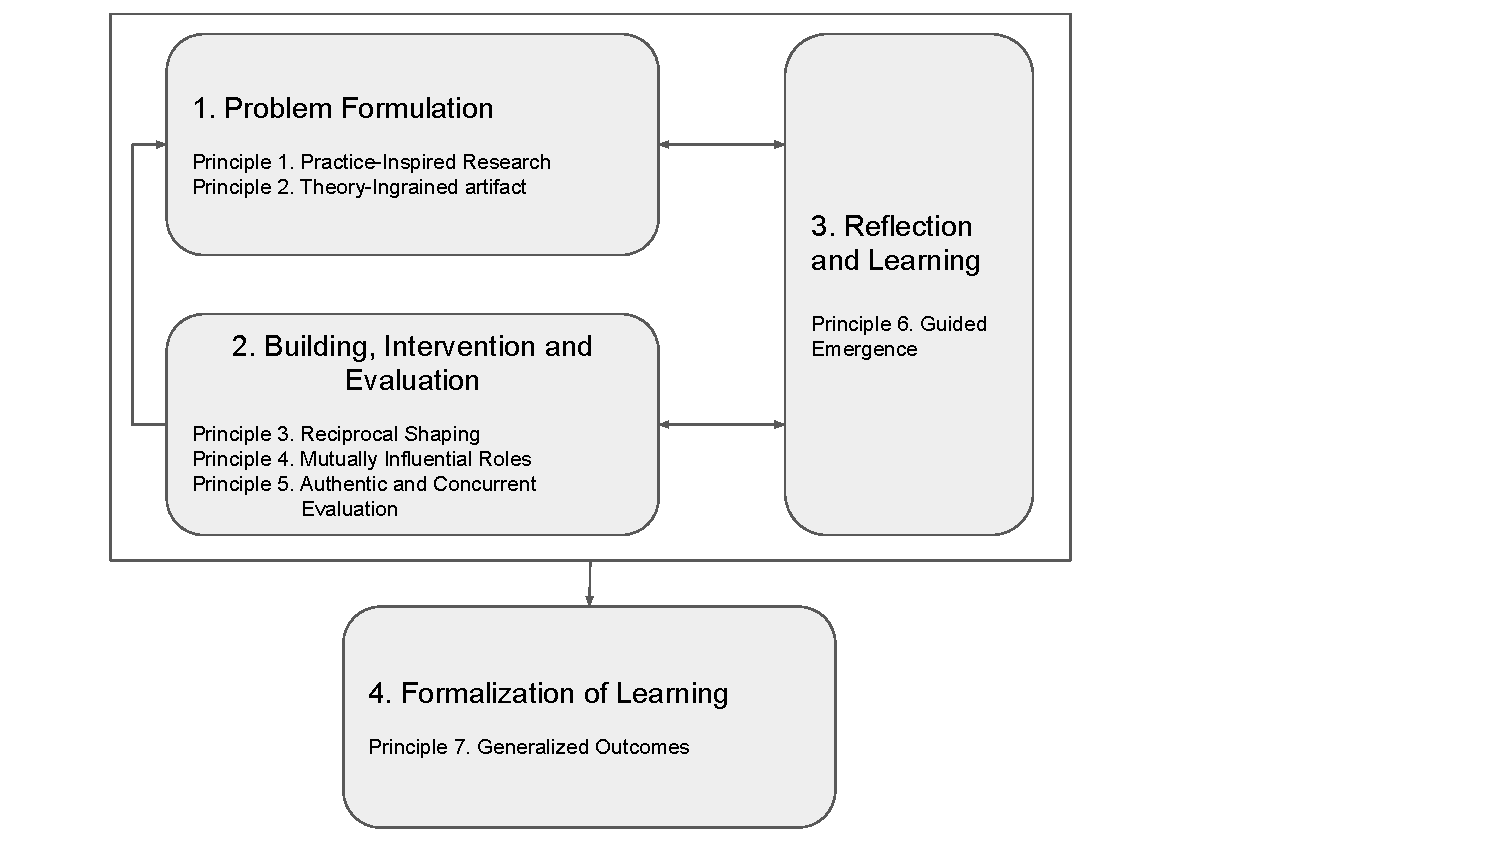
\includegraphics[width=12cm]{diagram/Action_Design_Research_Reproduced.pdf}
\caption{Action Design Research stages and principles \citep[reproduced following][]{Sein2011ActionResearch}}
\label{fig:adr-stages-and-principles}
\end{figure}

% Analogously, \cite{Vaishnavi2007} introduce the General Design Cycle (GDC) to drive any DSR process. The GDC process begins from the awareness of the problem and continues to one or more suggestions for solution. Next, an implementation of the plan is developed and evaluated, and finally, the process is concluded and the results shared; in the case of a scientific process, they are published. In each of these steps, new knowledge is both created and fed back to previous phases. The phases are repeated in an iterative fashion until a satisfactory end result (one that has practical utility) is achieved.

ADR stresses the importance of iteration and interaction with the future users of the IT artifact. The interaction is enabled by the Building-Intervention-Evaluation (BIE) cycle where an artifact is Built and used to implement an Intervention in an organization and to Evaluate the artifact over several BIE cycles. To develop the guidelines for investigating innovation ecosystems as networks as well as the Ostinato Model, we repeat the BIE cycle over series of experiments described in detail in Chapter~\ref{ch:experiments}. The BIE cycle allows us to evaluate the Ostinato Model for validity and added credibility of the presented results. Through guided emergence, we are able to contribute to innovation ecosystem research with deep knowledge of the problem and the proposed solution.

\cite{Sein2011ActionResearch} note that while DSR separates artifact building and evaluation, ADR emphasizes the iterative nature of artifact development. ADR is, therefore, well in line with the principles of contemporary software development approaches. Readers with experience in software development will indeed notice a straightforward connection between the BIE cycle and agile software development \citep[see e.g.][]{Schwaber2001}. More recently, startups and other value-seeking communities within the software development industry have turned their attention to Lean Startup, another iteration-based method \citep{Ries2011}. Apart from the intent to publish the results, these three design and development processes move forward in an iterative and incremental fashion and are guided by feedback collected from the users and other stakeholders of the developed software or other artifact, here the process model.

Design science sometimes receives critique for the lack of scientific rigor or bias in practice over theory. ADR responses with the principle of Authentic and Concurrent Evaluation \citep{Sein2011ActionResearch} that we apply through this dissertation. 
% Moreover, to further add to the rigor of the presented research, we will evaluate the research outputs following the core evaluation criteria for qualitative research: credibility, transferability, dependability, and confirmability \citep{Jussila2015SocialInnovation} \todo{Add more references including Guba (1981), Denzin and Lincoln (2000), and Shenton (2004).} 
The utility and viability of artifacts created with the DSR process can be evaluated through proof-of-concept, proof-of-value, or proof-of-use \citep{Nunamaker2011TowardSystems}, each of which adding to the requirements for the state of the artifact as well as the potential level of insight that the artifact has the ability to create.  

\section{Outline and contributions of the dissertation}
\label{sec:structure}

This dissertation is composed of two complementing lines of investigations. First, a series of experiments on innovation ecosystem investigations using visual network analytics is presented. Second, the Ostinato Model, an exploration-automation cycle for a user-centric, process-automated, data-driven visual network analytics is induced and described.

This dissertation is divided into eight (8) chapters, preceded by the description of 7 articles that together with this summary and synthesis of results form the whole of the dissertation. The articles are attached in this dissertation. The contents of each chapter are described briefly below.

Chapter~\ref{chapter:intro} introduces the context of this dissertation, describes the research method and specifies the objectives and key contributions of the dissertation.

Chapter~\ref{ch:background} reviews the core literature on the key domains of the dissertation, namely innovation ecosystems, network analysis, and visual network analytics.

Chapter~\ref{ch:ecosystemnetworks} introduces the domain of the dissertation in more detail. We describe the concept of innovation ecosystems, present existing work on the analysis of innovation ecosystems as networks, and discuss the utility of network analysis for decision-making. 

Chapter~\ref{ch:experiments} walks through the results of the investigations from the point of view of data-driven visual network analytics. For brevity and tractability of the discussion, we concentrate in the specifics of how visual network analytics were approached in each of the investigations. 

Chapter~\ref{ch:ecosystemnetworks} creates a synthesis of the way to represent and analyze innovation ecosystems as networks on basis of the investigations as action design research experiments.

Chapter~\ref{ch:processmodels} presents a set of process model requirements stemming from the experiments and goes through existing process models that the Ostinato Model is built on. 

Chapter~\ref{ch:ostinato} describes the Ostinato Model for data-driven visual investigations of innovation ecosystem structure.

Chapter~\ref{ch:discussion} discusses the contributions of this dissertation and provides a synthesis of the key results of the dissertation.

Chapter~\ref{ch:conclusions} concludes the dissertation and presents directions for further work.
 
This research makes contributions in two complementing levels. First, a process model for conducting data-driven visual network studies is developed and described. Second, a series of investigations in the field of innovation ecosystem exploratory analysis is conducted, feeding new insights into the emerging phenomena of innovation ecosystems and their research. A concrete outcome of the second contribution is the list design guidelines for representing innovation ecosystems as networks.

In terms of increasing the transparency of the structures emerging from individual transactions and affiliations between innovation ecosystem actors, this dissertation contributes in three levels. First, network analysis is a key approach in supporting exploratory studies on the patterns and structures in between actors founding, working for, advising and investing into startups and growth companies; companies making deals and alliances, investing into and acquiring other companies; and financial organizations investing into startups and growth companies  and in estimating the authority, role and structural position these actors have, therefore allowing for increasing the transparency of the structure of innovation ecosystems of different levels of abstraction from platforms, programs and business sectors to national and international innovation ecosystems. These structures can be modeled, represented, analyzed and visualized as networks to support the investigations and exploration. Second, the presented data-driven approach allows extending these investigations of patterns and structures within and in between groups of actors beyond the boundaries of individual datasets and to happen over long periods of time. Third, actors with different sets of skills from means to crawl online sources for data to domain knowledge allowing deep sensemaking can all fully engage into the different phases of the investigative process.

Moreover, investigations on innovation ecosystems contribute to the body of knowledge on the domain of innovation ecosystem studies with an empirical approach. At the same time, these investigations serve as a vehicle for developing the process model in an incremental and iterative manner following the Action Design Research process.
 
The main contributions of this research are as follows:

\begin{enumerate}[label=\textbf{Contribution \Roman*},align=left]
  \item To meet \ref{objective:empirical}, we contribute to the empirical body of knowledge with a visual description of innovation ecosystems in platform, program, business domain, national and international level through a series of investigations. 
  \label{contribution:empirical}

  \item To answer \ref{objective:ecosystemnetworks}, we define a set of design guidelines for modeling and analyzing the structure of innovation ecosystems as networks to support their exploratory analysis.
  \label{contribution:ecosystemnetworks}
   
  \item To satisfy \ref{objective:processmodel}, we define the Ostinato Model for data-driven visual network analytics in the context of innovation ecosystems.
  \label{contribution:processmodel}
\end{enumerate}

% \todo{Link the contributions to specific chapters or sections in the dissertation}

The key result of this dissertation is the introduction of the process model for data-driven visual network analytics in the context of innovation ecosystem investigations. The model is described in detail in \ref{pub:ostinato}.